\section{\sysname}
\label{sec:design}
Our design for \sysname focus on avoiding costly, unnecessary invocations of the network stack.
Envoy prides itself on being application agnostic, which leads to the helpful ability to auto-inject Envoy into microservices.
However, this abstract requires unnecessary invocations of the network stack.
In Figure-\ref{fig:no_kmap} we highlight in red all the calls to the network stack for the path of a single request.
Then, in Figure-\ref{fig:kmap} we show the reduction in those calls by using Kmap instead of the network stack for local data transfer.

\sysname works by using LD\_PRELOAD to load augmented network calls before libc regular calls.
Then, when Envoy and the microservice invoke read or write calls locally, rather than passing the data
into the network stack, we use \sysname's shared buffers to efficiently transfer the data.
Thus, we must load the shared library for both the Envoy sidecar and the microservices.
The two critical challenges to realizing \sysname are:
\begin{enumerate}
    \item Building a robust, efficient shared buffer \textit{faster} than the network stack
    \item Determining in a microservice-agnostic way which socket calls should use \sysname
\end{enumerate}

\begin{figure}[!htb]
    \begin{minipage}{0.5\textwidth}
        \centering
        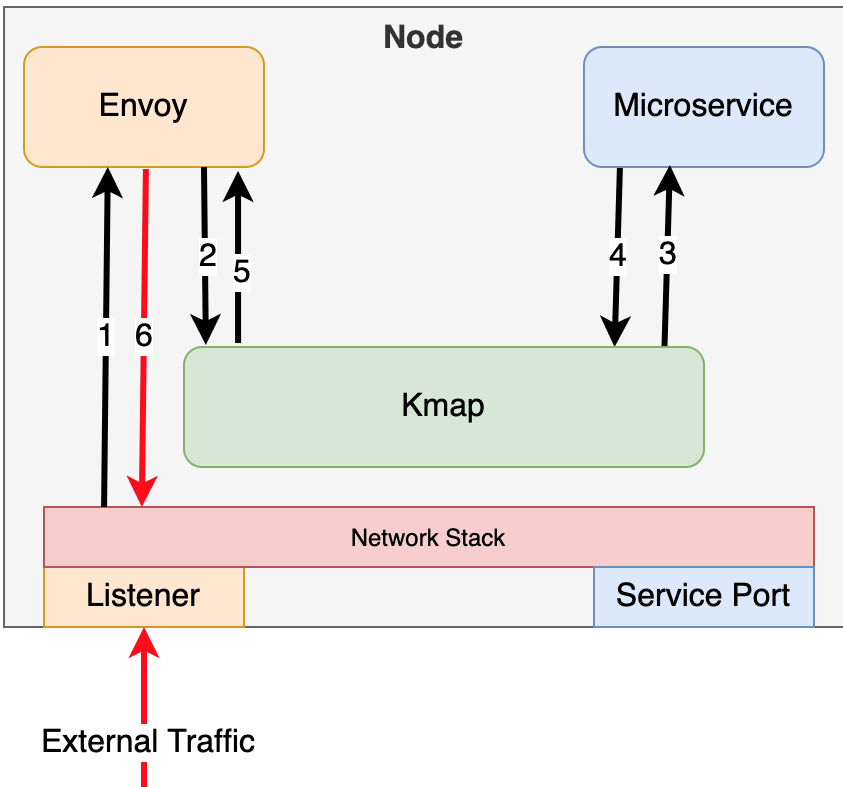
\includegraphics[keepaspectratio=true,width=3in]{figures/design/kmap.png}
        \caption{Kmap}
        \label{fig:kmap}
    \end{minipage}%
\end{figure}

\subsection{LD Preload}



\subsection{Pipe options}
Here, we outline potential methods for implementing the buffer \sysname uses to pass data between Envoy and the microservice.


\textbf{Named Pipes:}
Named pipes, (FIFO) are blocking, uni-directional I/O buffers for passing data between two processes.
The pipe must be opened for both reading and writing before being written two.
Named pipes are traditionally slow, only offering slight speed advantages over TCP.
Further, they are un-directional which makes them less accessible or interchangeable compared to TCP.

\textbf{Unnamed Pipes:}
Unnamed pipes are slightly faster than Named pipes, but are created per-process.
They traditionally are used when a process forks, as they both will share a reference to the pipe.
This makes them particularly tricky to implement across two independent processes and thus unhelpful for \sysname.

\textbf{Shared Memory:}
Shared memory is a robust API which allows processes to share use of a memory region (\textit{schm\_open}).
This requires mapping the same underlying memory region into the virtual memory of each process (\textit{mmap}).
Shared memory is concretely faster than pipes and the primary API \sysname uses for communicating information.
Shared memory has been benchmarked to be 170 times faster than TCP sockets for communicating information between processes.
However, shared memory does not directly provide a buffer interface like TCP, ans so \sysname must implement that as part of its library.


\subsection{When to apply \sysname}
The network stack has a very well defined, robust API which applications use to communicate.
A particular challenge for \sysname is pre-loading in front of those network calls and knowing when
to pass through the call, or when to route to the local buffer.
Since \sysname is designing primarily for Envoy, we use information about how it communicates with microservices to determine
which file descriptors should use \sysname.
This approach is not directly applicable to other sidecars (i.e. Linkerd) but is generalizable for applications, provided the applications work with Envoy first.


